\makeatletter\frontmatter@init\makeatother

\title{On-chip microwave quantum Hall circulator}

	\author{A. C. Mahoney}
	\author{J. I. Colless}
	\author{S. J. Pauka}
	\author{J. M. Hornibrook}
		\affiliation{ARC Centre of Excellence for Engineered Quantum Systems, School of Physics, The University of Sydney, Sydney, NSW 2006, Australia.}
		\affiliation{Station Q Sydney, The University of Sydney, Sydney, New South Wales 2006, Australia.}
	\author{J. D. Watson}
		\affiliation{Department of Physics and Astronomy, Purdue University, West Lafayette, Indiana 47907, USA.}
		\affiliation{Birck Nanotechnology Center, School of Materials Engineering and School of Electrical and Computer Engineering, Purdue University, West Lafayette, Indiana 47907, USA.}
	\author{G. C. Gardner}
		\affiliation{Birck Nanotechnology Center, School of Materials Engineering and School of Electrical and Computer Engineering, Purdue University, West Lafayette, Indiana 47907, USA.}
		\affiliation{Station Q Purdue, Purdue University, West Lafayette, Indiana 47907, USA.}
	\author{M. J. Manfra}
		\affiliation{Department of Physics and Astronomy, Purdue University, West Lafayette, Indiana 47907, USA.}
		\affiliation{Birck Nanotechnology Center, School of Materials Engineering and School of Electrical and Computer Engineering, Purdue University, West Lafayette, Indiana 47907, USA.}
		\affiliation{Station Q Purdue, Purdue University, West Lafayette, Indiana 47907, USA.}
	\author{A. C. Doherty}
		\affiliation{ARC Centre of Excellence for Engineered Quantum Systems, School of Physics, The University of Sydney, Sydney, NSW 2006, Australia.}
	\author{D. J. Reilly}
		\affiliation{ARC Centre of Excellence for Engineered Quantum Systems, School of Physics, The University of Sydney, Sydney, NSW 2006, Australia.}
		\affiliation{Station Q Sydney, The University of Sydney, Sydney, New South Wales 2006, Australia.}

\makeatletter
\begingroup
\@author@finish
\frontmatter@author@produce@script
\endgroup
\makeatother

\begin{abstract}
	Circulators are non-reciprocal circuit elements integral to technologies including radar systems, microwave communication transceivers, and the readout of quantum information devices. Their non-reciprocity arises from the interference of microwaves over the centimetre-scale of the signal wavelength, in the presence of bulky magnetic media that breaks time-reversal symmetry.
	Here we realize a completely passive on-chip microwave circulator with size 1/1000th the wavelength by exploiting the chiral, `slow-light'  response of a 2-dimensional electron gas (2DEG) in the quantum Hall regime. For an integrated GaAs device with \SI{330}{\micron} diameter and approximately \SI{1}{\giga\hertz} centre frequency, a non-reciprocity of \SI{25}{\decibel} is observed over a \SI{50}{\mega\hertz} bandwidth. Furthermore, the non-reciprocity can be dynamically tuned by varying the voltage at the port, an aspect that may enable reconfigurable passive routing of microwave signals on-chip.
\end{abstract}

\subsection{Introduction}
Miniaturized, non-reciprocal devices are currently of broad interest for enabling new applications in acoustics \cite{fleury2014sound}, photonics \cite{feng2011nonreciprocal,bi2011chip}, transceiver technology \cite{estep2014magnetic}, and in the regime of near quantum-limited measurement \cite{stace2004mesoscopic,kerckhoff2015chip,abdo2013directional,sliwa2015reconfigurable,PhysRevX.4.021019}, where they are needed to isolate qubits from their noisy readout circuits.
Since the 1950s, passive circuit elements exhibiting non-reciprocity at microwave frequencies have been implemented using bulky magnetic devices that are comparable in scale to the centimetre wavelength of signals in their operating band. The footprint of these components poses a major limitation to integrating entire systems on a chip, such as what is required, for instance, to scale-up quantum computing technology.

A seemingly obvious means of realizing non-reciprocity on a semiconductor chip is to use the Hall effect, where an external magnetic field breaks the time reversal symmetry of electrical transport \cite{mason1953hall}. Hall-based devices were ruled out in 1954 however \cite{wick1954solution}, since near the electrical contacts, where the current and voltage are collinear, dissipation is so significant that the usefulness of this approach is greatly limited. This dissipative mechanism has an analog in the quantum Hall regime where the two-terminal resistance of a device is always finite over a scale of the inelastic scattering length as carriers transition from their contacts to the dissipationless, one-dimensional (1D) edge-states that support transport \cite{buttiker1988absence}. Recently, Viola and DiVincenzo \cite{PhysRevX.4.021019} have proposed a means of addressing the limitation imposed by 2-terminal dissipation, suggesting the possibility of coupling microwave signals to the edge of a quantum Hall device reactively, without using traditional ohmic contacts. In a geometry where the signal ports of the device are positioned orthogonal to an incompressible quantum Hall edge-state, microwave power is coupled capacitively and non-dissipative transport in one-direction appears possible \cite{PhysRevX.4.021019}.

Here we engineer, on-chip, a chiral microwave interferometer that yields a high degree of non-reciprocity and dynamic range, with the low-dissipation inherent to edge transport in the quantum Hall regime. Configured as a completely passive 3-port circulator, our device demonstrates non-reciprocal operation at frequencies and magnetic fields commonly used for the read out of spin qubits \cite{Reilly:2007ig,barthel2009rapid, PhysRevLett.110.046805, nature11449}, facilitating integration with such semiconductor technologies. In comparison to traditional ferrite-based microwave components, this quantum Hall circulator is reduced in size by a factor of $\sim$ 1/1000th the wavelength and exhibits a new mode of operation in which circulation can be dynamically reconfigured either by applying a dc voltage to the port electrodes, or by altering the strength of the magnetic field. A simple model based on a Fano-resonance mechanism \cite{miroshnichenko2010fano} qualitatively accounts for the observed phenomena.

\subsection{Experimental Setup and Results}
\subsubsection{Transmission line spectroscopy of EMP modes}
\begin{figure}
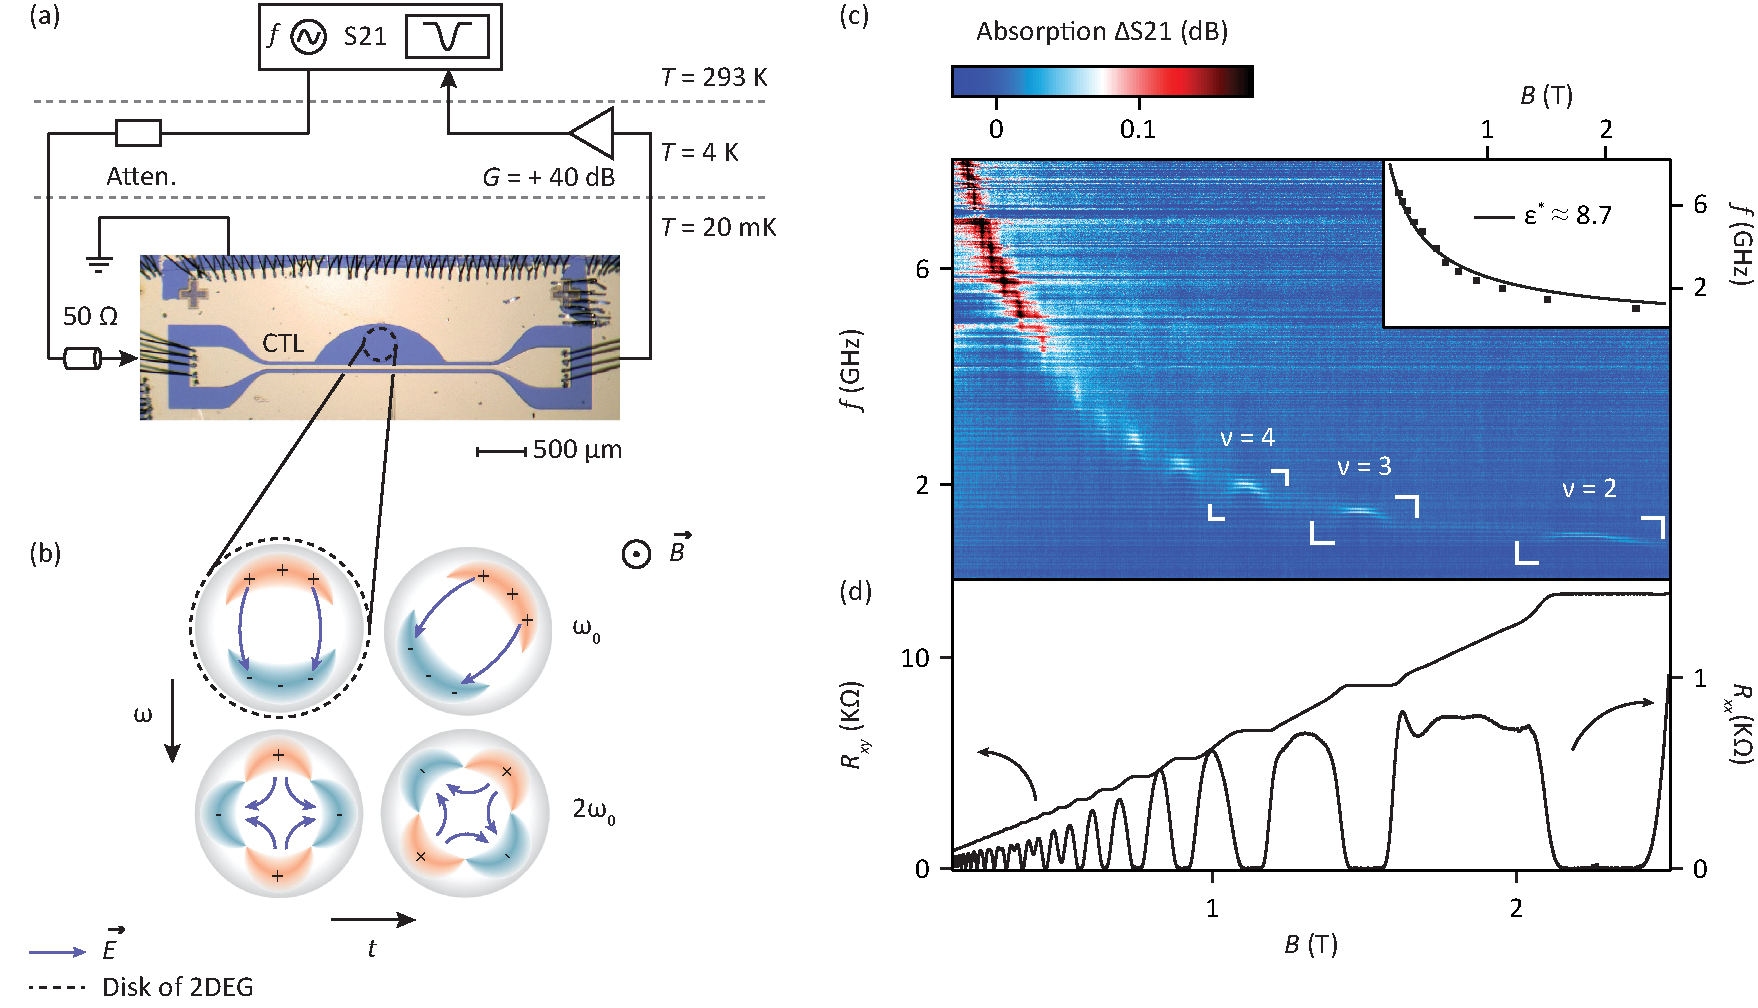
\includegraphics[width=\textwidth]{fig1_QH}
\caption[Detecting microwave edge magnetoplasmons (EMPs)]{\label{FIG. 1.}
(a) Experimental setup including photograph of a coplanar transmission line device similar to that used to perform measurements coupled to a \SI{330}{\micron} etched disc of 2DEG (black dashed circle) at fridge temperature $T = \SI{20}{\mk}$. A vector network analyser is used to excite EMP modes across a wide frequency range and microwave absorption is measured as the ratio of the amplified output to input signal ($S_{21}$) from the CTL.
(b) Illustration of the fundamental (top row) and first harmonic (bottom row) EMP modes as they evolve with time, where $\omega_0$ is the fundamental mode and $2 \omega_0$ the first harmonic (adapted from \cite{1988ZhETF..94..217V}). Charge distributions and electric fields $\vec{E}$ are indicated schematically. An external magnetic field $B$ applied to the device points out of the page.
(c) EMP spectrum of the quantum Hall disk showing absorbed microwave power as a function of frequency and magnetic field. Data has had a background, obtained at high field, subtracted. Inset shows the position of absorption dips at integer quantum Hall filling factors. Black line is a fit that allows an average effective dielectric constant of $\epsilon^{*} \approx 8.7$ to be extracted, consistent with excitations of an edge-state in GaAs (see supplementary material).
(d) Transverse ($R_{xy}$) and longitudinal ($R_{xx}$) Hall resistance measurements taken at $T = \SI{20}{\mk}$ on a Hall bar proximal to the microwave disk. The 2DEG is \SI{270}{\nano\meter} below the surface with carrier density $n_s$ = \den{1.1e11}, and mobility $\mu$ = \mob{5.2e6}.}
\end{figure}

Central to the operation of our device are edge magnetoplasmons (EMPs), resonant modes of the electron gas first observed in the classical response of electrons on the surface of liquid Helium \cite{PhysRevLett.54.1706, glattli1985dynamical}. Such excitations have since been found to propagate along a quantum Hall edge in response to a capacitively coupled microwave excitation \cite{1988ZhETF..94..217V, andrei1988low, talyanskii1990edge, ashoori1992edge,zhitenev1994experimental, kumada2013plasmon, petkovic2013carrier, kumada2014resonant}. These chiral excitations travel with a velocity $v_{EMP}\sim|\vec{E}|/|\vec{B}|$,  set by the ratio of the electric field $\vec{E}$ at the sample boundary and the applied magnetic field $\vec{B}$ \cite{talyanskii1990edge}.

For a high mobility 2DEG formed at the interface of the semiconductors GaAs and AlGaAs (see supplementary materials for details), the velocity of the EMP modes is typically $v_{EMP}\sim \SI{e5}{\meter\per\second}$ \cite{kumada2011edge, kamata2010voltage}, some 1000 times slower than the speed of light in the semiconductor dielectric. In order to exploit these EMPs to realize non-reciprocal microwave devices, we first detect their presence in a contactless etched disk of quantum Hall fluid by coupling to a proximal metallic coplanar transmission line (CTL) \cite{cano2013microwave}, as shown in Fig. \ref{FIG. 1.}(a) and \ref{FIG. 1.}(b). By measuring the transmitted microwave power through the CTL as a function of frequency $f$, a spectrum of discrete features is observed with applied magnetic field $B$ (Fig. \ref{FIG. 1.}(c)). We identify EMP modes in the data with frequencies set by the edge velocity and circumference of the disk, following the dependence $f\sim B^{-1}(\log(B^2) + \textrm{const.})$ \cite{1988ZhETF..94..217V}, and extract the effective dielectric constant $\epsilon^* \approx 8.7$ consistent with the propagation medium \cite{ashoori1992edge,balaban1997observation} (see supplementary materials). Comparing the microwave spectrum to transport measurements from a Hall bar on the same chip (Fig. \ref{FIG. 1.}(d)), we note that at high field (with only the last few Landau levels occupied) features resolve into discrete, crescent-shaped resonances that coincide with minima in the longitudinal resistance $R_{xx}$, where dissipation is suppressed.

\subsubsection{3-Port circulator}
\begin{figure}
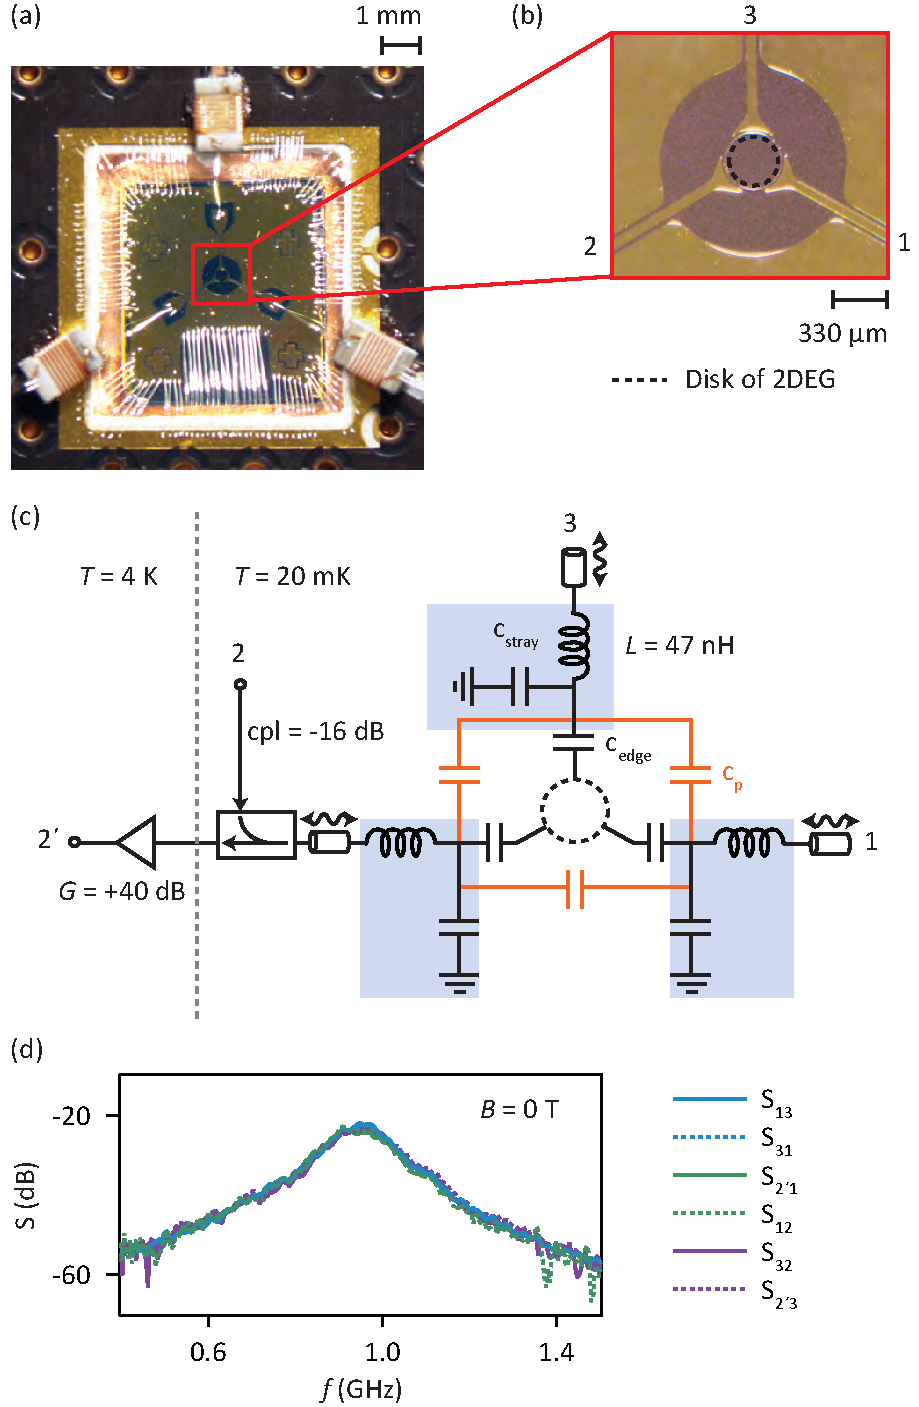
\includegraphics[width=0.7\columnwidth]{fig2_QH}
\caption[Experimental setup for determining the response of the on-chip circulator]{\label{FIG. 2.}
(a) Photograph of circulator device showing the three coplanar transmission lines connected to copper wire-wound chip inductors for impedance matching.
(b) Close-up of false-coloured photo of the circulator showing \SI{330}{\micron} diameter 2DEG disc with a \SI{20}{\micron} gap to the metal defining the three signal ports.
(c) Circuit schematic of the experimental setup indicating port-to-edge capacitive coupling $C_{\rm edge}$ and direct parasitic coupling between ports $C_{\rm p}$. Resonant ($LC_{\rm stray}$) matching circuits are indicated with blue boxes. The input of port 2 passes through a directional coupler, with the reflected signal coupled to the output line (denoted $2^\prime$) and amplified at \SI{4}{\kelvin}.
(d) Full 6-way transmission response of the circulator at zero magnetic field, with $S$-parameter measurements indicating complete reciprocity and a frequency response that arises from the matching networks. For each port the measured response of the amplifiers, couplers and cold attenuators in the circuit have been subtracted.}
\end{figure}

To test if these edge magnetoplasmons support the non-reciprocal transmission of microwaves, we implement a standard circulator configuration, with 3 ports arranged at 120-degree intervals around a disk of 2DEG (\SI{330}{\micron} diameter), as shown in Fig. \ref{FIG. 2.}(a) and \ref{FIG. 2.}(b). For a single edge at high magnetic field, a voltage applied to a port capacitance induces an orthogonal current in the edge-state, with an impedance of the order of the inverse conductance quantum ($\sim \SI{26}{\kilo\ohm}$). Given our present measurement setup uses electronic components with a characteristic impedance of $Z_0 \sim \SI{50}{\ohm}$, we have added an impedance matching circuit to enhance the response of each port. This network comprises a series chip-inductor $L = \SI{47}{\nano\henry}$ in resonance with the stray capacitance $C_{\rm stray}$. The impedance of the Hall edge could be lowered closer to $Z_0$ by connecting multiple 2DEG circulators in parallel \cite{druist1998observation}, or by taking advantage of recently proposed `self-matching' port configurations \cite{bosco2016self,placke2016model} (see supplemental materials for detailed discussion). The circulator is also embedded in a reflectometry arrangement (Fig. \ref{FIG. 2.}(c)) that enables a measurement of the port reflection as well as port transmission coefficient, from which dissipation can be estimated. As a control we first measure all microwave $S$-parameters at zero magnetic field, observing that all directions and ports are equivalent, as shown in Fig. \ref{FIG. 2.}(d).  An overall frequency-dependent, but reciprocal response can be associated with the impedance matching network, with matching frequency set to $1/\sqrt{LC_{\rm stray}} \sim \SI{1}{\giga\hertz}$.  All subsequent measurements are normalized relative to this zero-field transmission response.

\begin{figure}
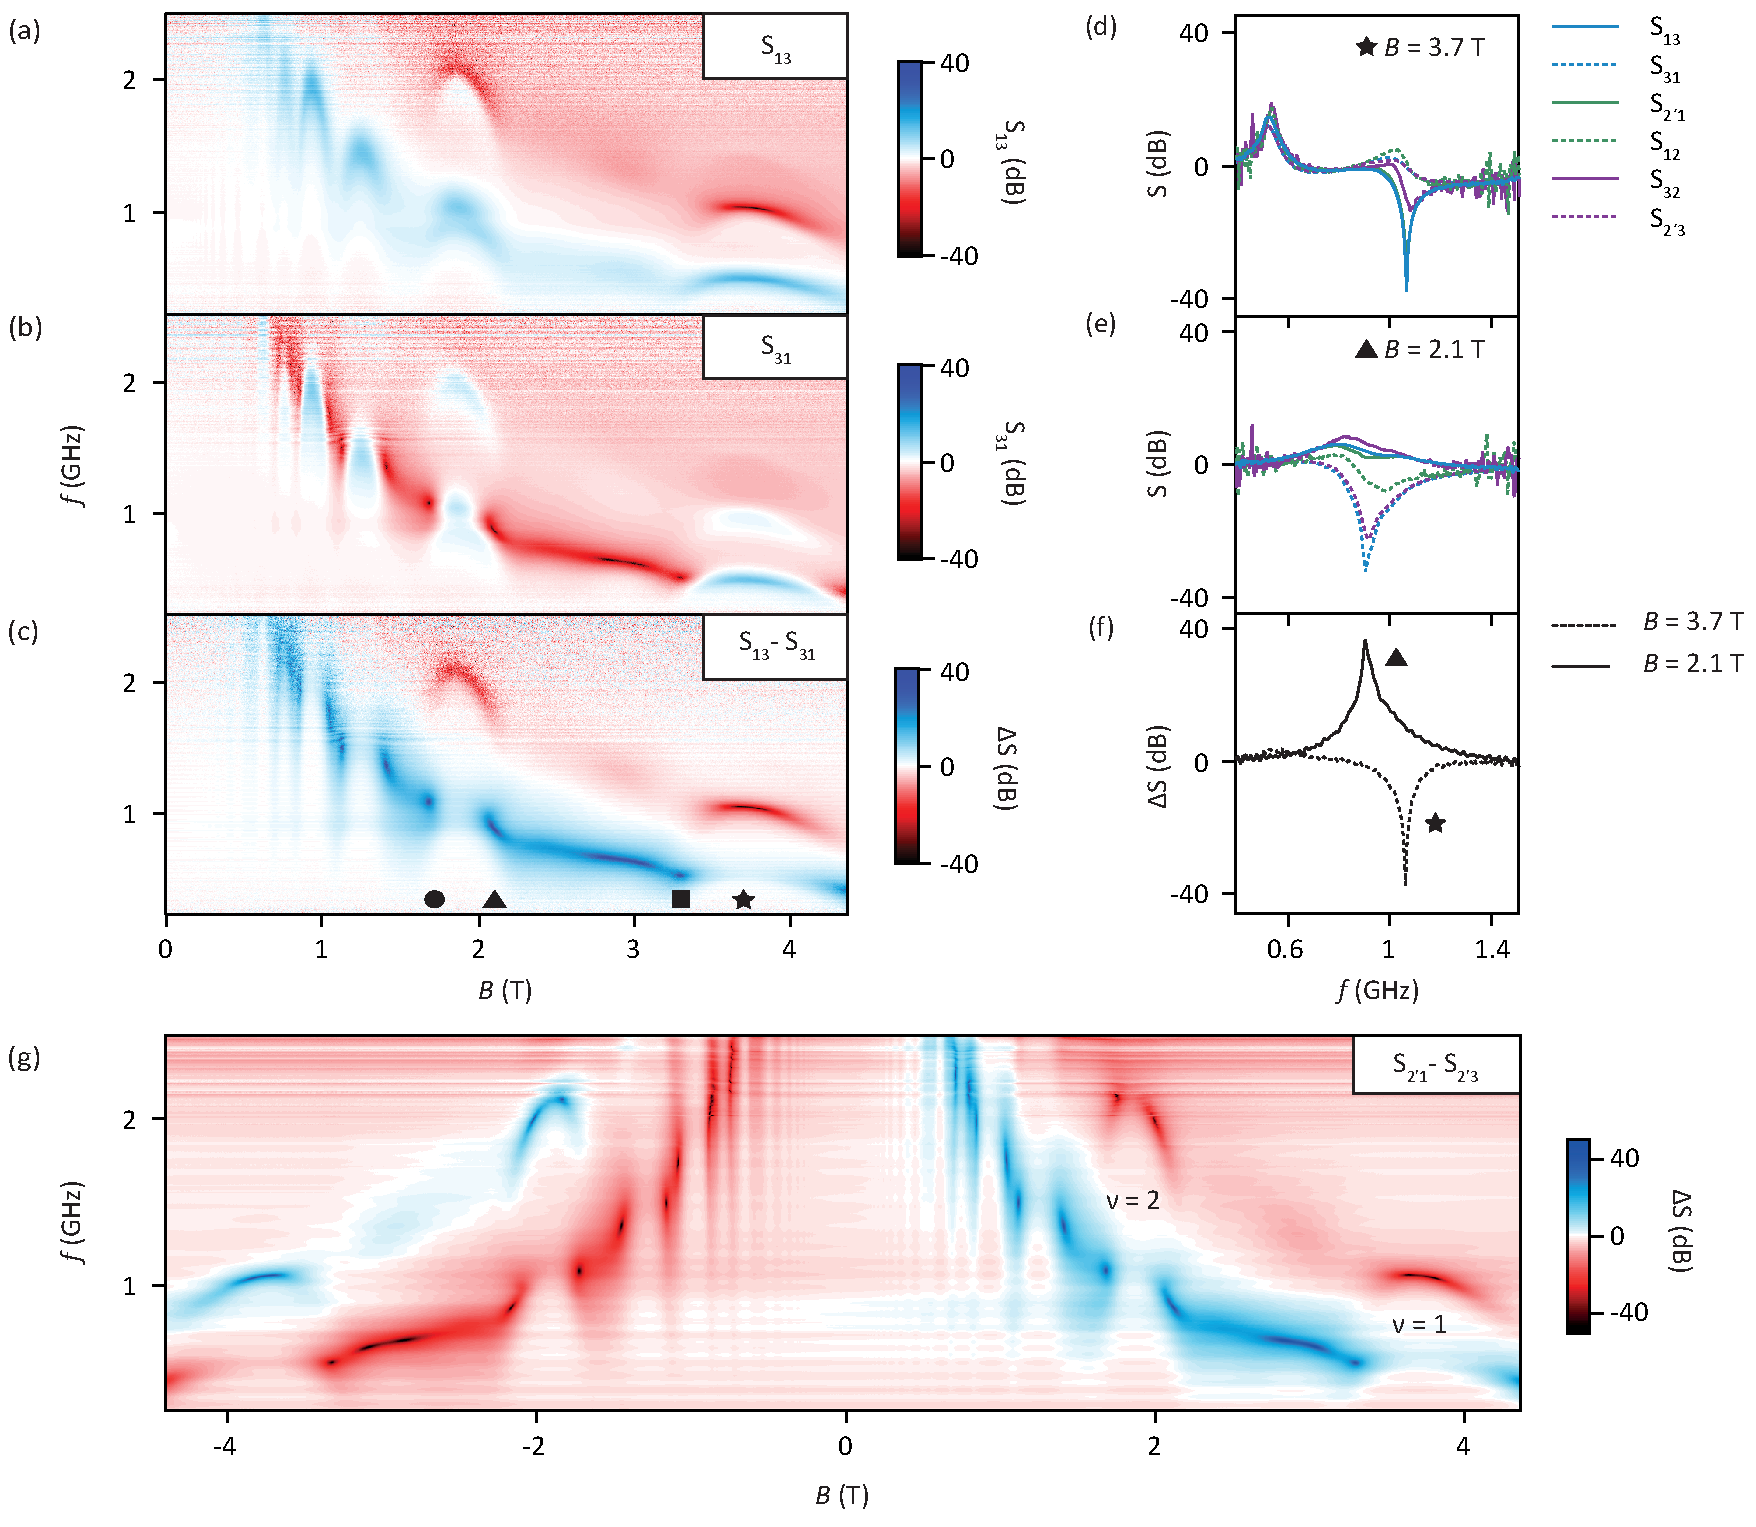
\includegraphics[width=\textwidth]{fig3_QH}
\caption[Non-reciprocal response of the quantum Hall circulator]{\label{FIG. 3.}
(a) and (b) Port transmission $S_{13}$ and $S_{31}$ with frequency and magnetic field. All measurements have been normalized to the gain-corrected background at $B = 0$ (shown in Fig. 2(d)), which defines the \SI{0}{\decibel} point on the colour scale.
(c) Microwave response $S_{13}-S_{31}$ showing strong frequency and $B$-dependent non-reciprocity.
(d) and (e) Full combination of transmission $S$-parameters, taken at $B$-fields indicated by the symbols in (c).
(f) Cuts through the colour scale data in (c), demonstrating forward and reverse circulation.
(g) Isolation, $\Delta S = S_{2'1}-S_{2'3}$, measured at positive and negative magnetic fields. Note that the positions of features are symmetric about the $B = 0$ axis, but with opposite sign $\Delta S$.}
\end{figure}

Turning to our key result, Fig. \ref{FIG. 3.} shows the full transmission response of the 3-port circulator in the presence of a magnetic field that breaks time-reversal symmetry. Similar to the EMP spectrum of Fig. \ref{FIG. 1.}(c), we first observe the presence of EMPs which enhance the transmitted power at certain frequencies, broadly following an approximate $f \sim B^{-1}$ dispersion relation, as is seen in Fig. \ref{FIG. 3.}(a) ($S_{13}$) and \ref{FIG. 3.}(b) ($S_{31}$). Strikingly, there are regions of the spectrum where the transmitted power appears to flow in either a forward or reverse direction with respect to the chirality of the edge. Particularly apparent are the crescent-shaped features that switch from forward to reverse transmission at distinct frequencies. This phenomenon, with a peak near the fundamental frequency of the EMP mode and a dip near the first EMP harmonic, is seen for all $S$-parameters in the chiral (clockwise) direction of the 3-port device (see solid lines in Fig. \ref{FIG. 3.}(d)).

To measure the extent of non-reciprocity in our circulator, Fig. \ref{FIG. 3.}(c) shows the difference between forward and reverse power by subtracting $S_{31}$ from $S_{13}$. Unlike the $B = 0$ data shown in Fig. \ref{FIG. 2.}(d), we now observe a strong directional dependence in the isolation between ports, that approach \SI{40}{\decibel} at particular frequencies and magnetic fields (Fig. \ref{FIG. 3.}(f)). Alternatively, we can also test for non-reciprocity by comparing the response of signals from two different inputs of the circulator to a common output. Since the device is geometrically symmetric, the response from the separate paths $S_{2'1}$ and $S_{2'3}$ are the same at $B = 0$, (see Fig. \ref{FIG. 2.}(d)). In the presence of a magnetic field however, Fig. \ref{FIG. 3.}(g) shows that these paths are no longer equivalent, but depend rather on the direction of the field. This is evident in the data since blue and red features are not mirrored about $B = 0$.

Comparing the microwave response of the circulator to independent quantum Hall transport data suggests  two distinct regimes. Between integer filling factors, where $R_{xx}$ is maximised in transport, there is a large non-reciprocity in the microwave response, but also likely strong dissipation. Contrasting these broad regions are narrow crescent-shaped features that occur at fields corresponding to integer filling. These narrow features are particularly strong at frequencies near twice the fundamental EMP resonance. Again, overlaying these features with transport measurements indicates they align with minima in $R_{xx}$, where dissipation is suppressed. A direct and accurate measurement of the microwave dissipation is challenging in the regime where the impedance of the device is mismatched. Nevertheless, by accounting for the transmitted and reflected signal power we find the dissipation to be a few percent, consistent with the value of $\sim 1\%$ given by our model (discussed below).

\subsection{Discussion and Model}
\begin{figure}
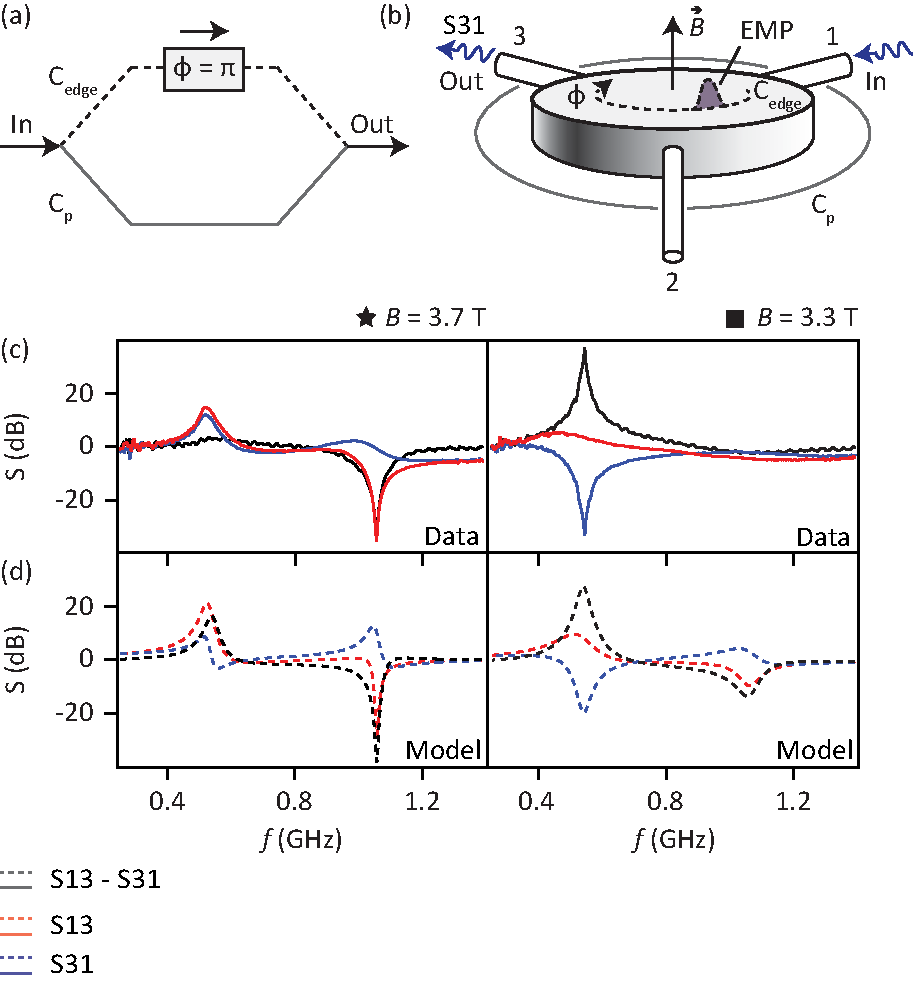
\includegraphics[width=0.7\columnwidth]{fig4_QH}
\caption[Comparison of data and model]{\label{FIG. 4.}
(a) and (b) Proposed interferometric mechanism underlying the operation of the quantum Hall circulator, with a slow plasmonic path, via $C_{\rm edge}$, and a direct capacitive path, via $C_{\rm p}$. A non-reciprocal response between ports is produced for frequencies where the two paths are out of phase by $\phi = \pi$ in the forward direction and $\phi = 2\pi$ in the reverse direction.
(c) and (d) Comparison of a simple model that captures this physics (top graphs), with experimental data (bottom graphs), at two different magnetic fields indicated by the symbols (with respect to Fig. \ref{FIG. 3.}(c)). The model is described in detail in the appendix with parameters set to values $Z_0 = \SI{50}{\ohm}$, $C_{\rm p} = \SI{315}{\femto\farad}$, $C_{\rm edge} = \SI{127}{\femto\farad}$, $R_{xy} = \SI{5000}{\ohm}$ with $R = \SI{80}{\ohm}$ in the centre of an EMP resonance (star symbol) and $R = \SI{350}{\ohm}$ off resonance (square symbol). Note that the impedance matching network transforms $R_{xy} = \SI{25}{\kilo\ohm}$ towards a few \si{\kilo\ohm}, consistent with the value used in the model.}
\end{figure}

We account for the distinct features in our measurements, as well as the phenomena of forward and reverse circulation via a simple picture of a Fano-like resonance. Figure \ref{FIG. 4.} illustrates the phenomenology of the quantum Hall circulator. Similar to the operation of a traditional ferrite device, we consider a resonator structure with two interfering paths, as shown in Fig. \ref{FIG. 4.}(a). The arms of this interferometer comprise a direct path, supported by the parasitic (geometric) capacitance $C_{\rm p}$ between ports, and an indirect path $C_{\rm edge}$, that capacitively couples ports via the plasmonic excitation of a quantum Hall edge. Key to the operation of our circulator is this `slow light' response of the EMP modes, which, traveling at velocities 1000 times slower than the microwaves in the direct path, acquire the same phase over a length scale that is 1000 times shorter than the microwave wavelength in the dielectric. Considering these two-paths we note that there will be a frequency near the EMP resonance, at which the phase acquired via the edge leads to complete destructive interference with the signal propagating via the direct path. Given the chirality of the EMP, the condition for destructive interference will be dependent on the direction of microwave transmission, producing a non-reciprocal response between adjacent ports. Take for instance, the case where signals from port 3 to 1 propagate clockwise via the edge capacitance $C_{\rm edge}$ and acquire a phase of $\pi$-radians with respect to the signal traveling via $C_{\rm p}$. Interference of these signals isolates port 1, whereas reverse transport, from port 1 back to port 3 must continue in a clockwise direction, past port 2 and acquire a constructive phase of $2 \pi$ over twice the length. Circulation in the opposite direction to the chirality of the edge can now be understood for frequencies in which a $\pi$-phase is acquired in the forward direction, but $2 \pi$-phase in reverse.

We construct a simple model based on this Fano-like picture of interfering paths \cite{miroshnichenko2010fano}, by modifying the standard response of a three-terminal Carlin circulator to account for transport via a quantum Hall edge (see Appendix). This yields an expression for the non-reciprocal admittance matrix of the edge, $Y_{\rm edge}$, as was done in Ref. \cite{PhysRevX.4.021019}. Extending the model in Ref. \cite{PhysRevX.4.021019}, we add an additional admittance term $Y_{\rm p}$ to account for a direct parasitic coupling $C_{\rm p}$ between terminals (see Fig. \ref{FIG. 2.}(c)). We further include the possibility of dissipation $R$, either directly in the chiral EMP mode or elsewhere in the circuit. Given an admittance of the edge-state $Y_{\rm edge}$, the total admittance is then given by:
\begin{equation}
	{Y_{{\rm{total}}}} = {({I} + R  Y_{\rm edge})^{ - 1}}Y_{\rm edge} + {Y_{{\rm{p}}}}
\end{equation}
where $I$ is the identity matrix and where
\[ {Y_{{\rm{p}}}} = \left( {\begin{array}{*{20}{c}}
{2c}&{ - c}&{ - c}\\
{ - c}&{2c}&{ - c}\\
{ - c}&{ - c}&{2c}
\end{array}} \right)\]
with $c = i\omega {C_p}$ and $\omega$ is the angular frequency of the microwaves. Microwave $S$-parameters can then be calculated as a function of $\omega$ for a given characteristic impedance of the input port ($Z_0$).

This model qualitatively captures the mechanism of circulation as arising from the interference of the parasitic and quantum Hall edge paths. Despite its simplicity, we find it also accounts for many of the features seen in the experimental data, including forward and reverse circulation that occurs near the fundamental and first harmonic of the EMP mode, as shown in Fig. \ref{FIG. 4.}(c) and \ref{FIG. 4.}(d). For features that occur at fields corresponding to integer filling, we find good agreement with the data for parameter values that are consistent with the device geometry and independent transport measurements (see Fig. \ref{FIG. 4.} caption for details). At magnetic fields slightly away from integer filling, increasing $R$ in the model yields similar results to the observed phenomena.

\subsection{Tunable non-reciprocity}
\begin{figure}
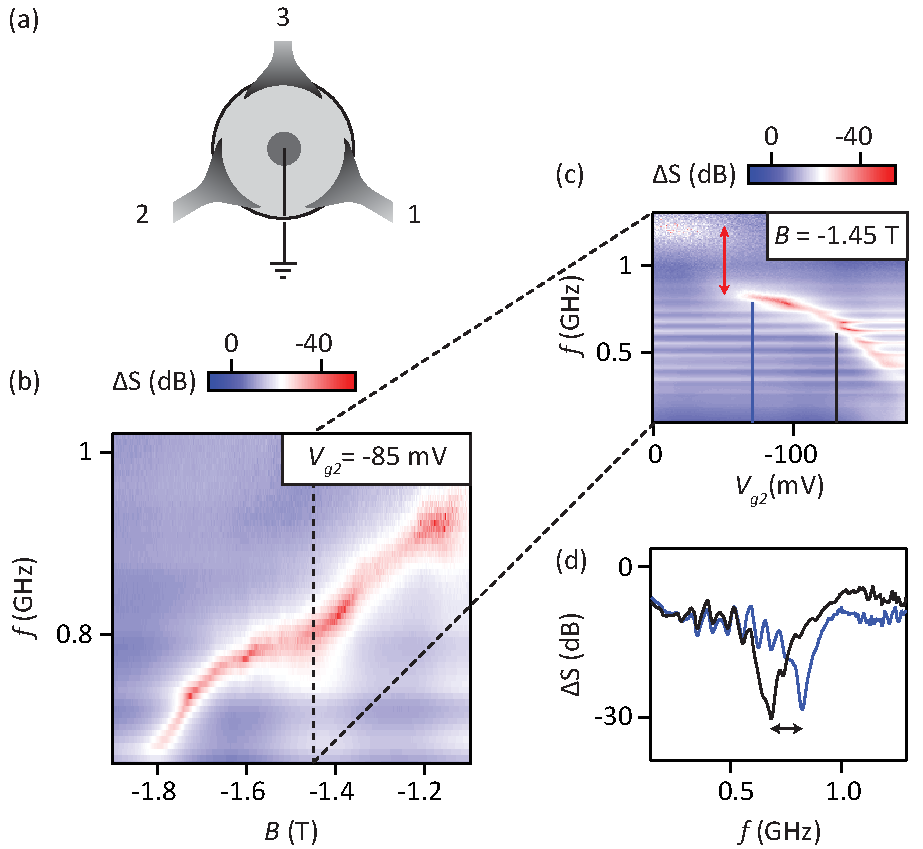
\includegraphics[width=0.75\columnwidth]{fig5_QH}
\caption[Tunable non-reciprocity of the quantum Hall circulator]{\label{FIG. 5.}
(a) Schematic of the gate-tunable device, with ports overlapping the edge of the disk and a grounded contact on the mesa. Bias tees enable the application of both rf and dc voltages.
A large non-reciprocity $\Delta S = S_{13}-S_{23}$ is observed as a function of magnetic field, as shown in (b) for the case $V_{g2} = \SI{-85}{\mv}$.
At fixed negative magnetic field values, varying $V_{g2}$ is found to affect the path from ports 3 to 1 and produces a significant modulation in the frequency response of the circulator (shown in (c) and (d)). This response is mirrored with a change of sign $\Delta S$ at positive magnetic field values, where the direction of EMP propagation is reversed and $V_{g1}$ is varied (see supplemental material).  Red arrow in (c)  indicates a discontinuous jump in frequency as a gate voltage is first applied, while vertical lines show the positions of 1D cuts presented in (d). Horizontal striations in (c) are the result of small standing waves associated with an impedance mismatch between the amplifier and device.}
\end{figure}

Finally, having outlined the mechanism leading to non-reciprocity in our device, we turn to describe a new mode that has no analog in the operation of classical circulators but may enable reconfigurable passive routing of microwave signals on-chip using gate voltages to modulate the velocity of EMPs. To demonstrate this mode we make use of an alternate device (Fig. \ref{FIG. 5.}(a)) where, in comparison to the previous device, the port electrodes are positioned to now overlap the edge and a grounded contact is added to the centre of the disk. Sweeping the magnetic field, we find this device exhibits regions of strong non-reciprocity, as shown in Fig. \ref{FIG. 5.}(b). Tunable non-reciprocity is demonstrated at fixed negative $B$-field by sweeping the dc voltage applied to the port-2 gate $V_{g2}$.  This adjusts the response between the source and sink ports 3 and 1 respectively, which tunes the frequency of isolation $\Delta  S  = S_{13}-S_{23}$ as shown in \ref{FIG. 5.}(c) and \ref{FIG. 5.}(d). Applying a voltage to a gate hardly modifies the total path length of the EMP in this geometry, but can lead to a significant modulation in its velocity by varying the carrier density, electric field, or extent of screening at the disk boundary \cite{kamata2014fractionalized,kumada2013plasmon}. As a function of $V_{g2}$, Fig. \ref{FIG. 5.}(c) shows that the non-reciprocal response of the circulator initially drops from $\sim \SI{1.2}{\giga\hertz}$ to $\sim \SI{0.8}{\giga\hertz}$ as the gate voltage is initially applied, followed by a more gradual decrease in the centre frequency as the gate is made increasingly negative. At present we do not understand why a modest gate voltage leads to a significant velocity modulation and therefore frequency response over such a large bandwidth (exceeding \SI{1}{\giga\hertz} and many line-widths in this device). An alternate means of reconfiguring the device can be achieved by adjusting the external magnetic field (as shown in the supplemental material).  In this way the circulator can produce forward or reverse circulation, selectively routing microwave packets to alternate ports depending on the value of the magnetic field. For such an application, generating the magnetic field on-chip using a combination of micromagnets \cite{pioro2008electrically} and compact superconducting solenoids could be considered.

\subsection{Conclusion}
We have demonstrated a compact, on-chip microwave circulator based on the non-reciprocal response implicit to the quantum Hall effect. With better matching between the port impedance and impedance of the quantum Hall edge, these highly-compact devices can immediately compete with today's commercially available bulky circulators circulators for cryogenic applications. To this end, we draw attention to recent theoretical works \cite{bosco2016self,placke2016model}  that suggest new configurations for achieving "self-matching" of the circulator to the characteristic impedance of the ports. Beyond the simple circulator devices demonstrated here, we conclude by noting that an edge-state can be considered as a mesoscale delay-line with dynamic, and gate-tunable wideband response. Such a dependence opens the prospect of compact, parametric devices such as amplifiers, non-reciprocal filters and mixers based on the plasmonic and chiral response of the quantum Hall effect. Indeed, such modes can also likely be realized at zero magnetic field using topological insulator devices that exhibit the quantum anomalous Hall effect \cite{chang2013experimental}.

\subsubsection{Acknowledgements}
We thank D. DiVincenzo, C. Nayak, and J. Cano for useful conversations. This research was supported by Microsoft Research, the US Army Research Office grant W911NF-14-1-0097, and the Australian Research Council Centre of Excellence Scheme (Grant No. EQuS CE110001013).